% This is samplepaper.tex, a sample chapter demonstrating the
% LLNCS macro package for Springer Computer Science proceedings;
% Version 2.20 of 2017/10/04
%
\documentclass[runningheads]{llncs}
%
\usepackage{graphicx}
\usepackage{todonotes}
\usepackage{amsmath}
\usepackage{theorem}
% Used for displaying a sample figure. If possible, figure files should
% be included in EPS format.
%
% If you use the hyperref package, please uncomment the following line
% to display URLs in blue roman font according to Springer's eBook style:
% \renewcommand\UrlFont{\color{blue}\rmfamily}

\begin{document}
%
\title{Result Quality of 3SAT\\on a Quantum Annealing Platform}
%
%\titlerunning{Abbreviated paper title}
% If the paper title is too long for the running head, you can set
% an abbreviated paper title here
%
\author{Thomas Gabor\inst{1} \and
Sebastian Zielinski\inst{1} \and
Sebastian Feld\inst{1} \and
Christoph Roch\inst{1} \and
Christian Seidel\inst{2} \and
Florian Neukart\inst{3} \and
Isabella Galter\inst{2} \and
Wolfgang Mauerer\inst{4} \and
Claudia Linnhoff-Popien\inst{1}}
%
\authorrunning{Gabor et al.}
% First names are abbreviated in the running head.
% If there are more than two authors, 'et al.' is used.
%
\institute{LMU Munich\and
??? \and
Volkswagen Group of America\and
OTH Regensburg}
%
\maketitle              % typeset the header of the contribution
%
\begin{abstract}
The abstract should briefly summarize the contents of the paper in
150--250 words.

\keywords{Quantum Computing \and Quantum Annealing \and 3SAT \and NP \and phase transition.}
\end{abstract}
%
%
%
\section{Introduction}
Following the great paper \cite{feld2018hybrid} we thought, let's do another one!
\todo{0.5 Introduction}

\section{Preliminaries}

\begin{figure}
\centering
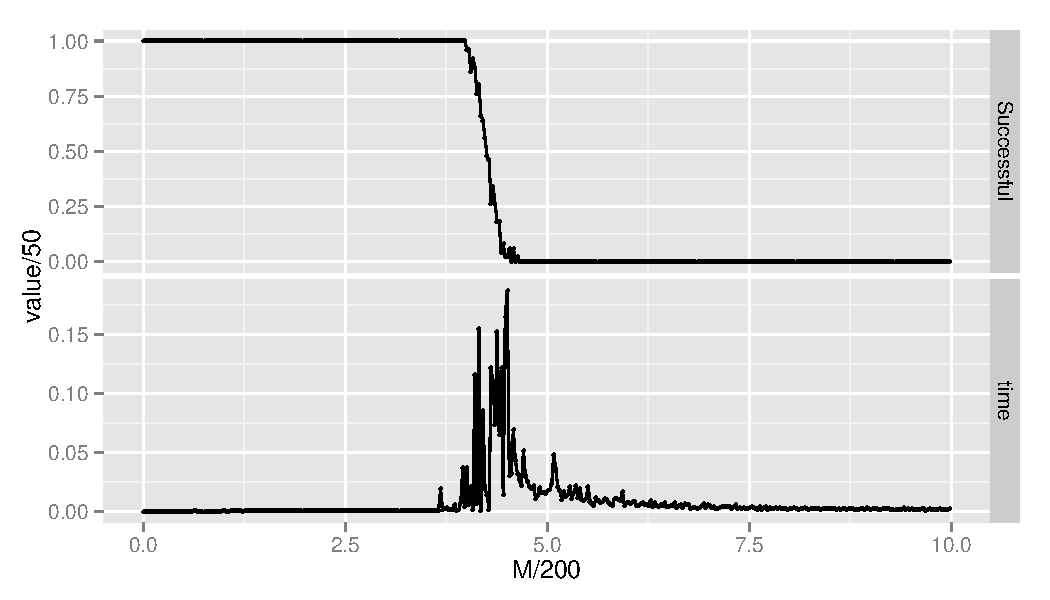
\includegraphics[width=.8\textwidth]{../material_2/plot_sat.pdf}
\caption{Loesungsfindungsdauer von 3SAT-Instanzen mit 1000 Klauseln für ver- schiedene Anzahl von Variablen.} \label{fig:distr}
\end{figure}


Das K - Erfüllbarkeitsproblem (im Folgenden\emph{ KSAT} genannt) gehört zur Klasse der NP-Vollständigen Probleme. KSAT ist, für K > 3, ein zentrales Problem in der kombinatorischen Optimierung und war das erste Problem, für das die NP-Vollständigkeit gezeigt werden konnte \cite{mezard2002random}.

Problembeschreibung: K - Erfüllbarkeitsproblem (nach  \cite{mezard2002random})
Gegeben sei eine Menge $\mathcal{B}$, bestehend aus N booleschen Variablen. Aus dieser Menge $\mathcal{B}$ werden dann K Variablen ausgewählt. Die ausgewählten Variablen, oder deren Verneinungen, werden dann durch (K-1) Oder-Operatoren zu einer \emph {Klausel} zusammengefasst. Auf diese Art und Weise werden M Klauseln gebildet. Durch anwenden von (M-1) Und - Operatoren entsteht so eine KSAT-Instanz.\\Das KSAT-Problem ist nun die Frage, ob eine Belegung der boolschen Variablen aus $\mathcal{B}$ existiert, so dass eine gegebene KSAT-Instanz erfüllbar ist.

In dieser Arbeit werden ausschließlich zufällig generierte KSAT-Instanzen für K=3 betrachtet. Diese Probleme werden dann 3SAT genannt und sind nach \cite{cook1971complexity} NP-Vollständing.

\subsection{Kritischer Punkt bei zufällig generierten KSAT-Instanzen}\label{krit:sat}
Bei zufällig generierten KSAT-Instanen kann beobachtet werden, die Wahrscheinlichkeit, eine korrekte Lösung für die Instanz zu finden, abrupt sinkt, wenn ein kritischer Wert $\alpha_{c}$ (gebildet aus dem Verhältnis von Anzahl der Klauseln zu Anzahl der Variablen) überschritten wird \cite{monasson1996entropy}.

Nach \cite{mezard2002random} liegt dieser kritische Punkt bei zufällig erzeugten 3SAT-Instanzen bei \\$\alpha_{c} \approx 4,267$. In der Umgebung des kritschen Punkts ist die Lösungsfindung (damit ist hier nicht nur eine konkrete Belegung gemeint, falls die Instanz lösbar ist, sondern auch die Erkenntnis, dass diese Instanz nicht gelöst werden kann) algorithmisch komplex. Abb. \ref{crit_sat} verdeutlicht dieses Phänomen visuell.

Zur Erstellung von Abb. \ref{crit_sat} wurden mit Hilfe des \emph{Tough SAT Generators}\footnote{https://toughsat.appspot.com/} 3SAT-Instanzen zu je 1000 Klauseln erstellt. Die Größe der  Menge der boolschen Variablen wurde ausgehend von 1000 schrittweise um 10 verringert, bis ein abschließendes Klausel zu Variablenverhältnis von ca. 7 erreicht wurde. Für jede Größe der so erzeugten Variablenmenge wurden 10 Instanzen erzeugt. Die verschiedenen Instanzen wurden dann mit dem SAT-Solver \emph{Minisat}\footnote{http://minisat.se/} gelöst. In Abb. \ref{crit_sat} ist dann einmal die durchschnittliche sowie die maximale Lösungsdauer der 10 Instanzen für ein bestimmtes Verhältnis dargestellt.
 %%%%%%%%%%%%%%%%% Maximum-Weight Independetn Set %%%%%%%%%%%%%%%%%%%%%%%%%%%%%%%%%%%%%%%%%%%%
\subsection{Das Problem der maximal gewichteten unabhängigen Menge}\label{chap:wmis}

--Unabhängige Menge \cite{feo1994greedy}]\label{def:unabhmenge}
Gegeben sei ein Graph $\mathcal{G} = (V,E)$, wobei V die Menge der Knoten des Graphs ist und E die Menge der Kanten des Graphs.\\Eine \emph{unabhängige Menge} von $\mathcal{G}$ ist eine Menge V' $\subset$ V mit folgender Eigenschaft:
\begin{equation}
(i,j) \notin E \;\;\;\forall i,j \in V' 
\end{equation}
Eine \emph{unabhänginge Menge} eines Graphen $\mathcal{G}$ ist also eine Teilmenge V' der Knoten von $\mathcal{G}$ so, dass die Knoten aus V' paarweise nicht direkt durch eine Kante von $\mathcal{G}$  verbunden sind.

--Maximal gewichtete unabhängige Menge \cite{choi2010adiabatic}
Gegeben sei ein ungerichteter Graph $\mathcal{G} = (V, E)$, wobei V die Menge der Knoten und E die Menge der Kanten von $\mathcal{G}$ sind, bei dem jeder Knoten v $\in$ V mit einem positiven reellen Gewicht $c_{v}$ versehen wird.\\
Das Problem ist es dann eine Menge S $\subset$ V zu finden, so dass S eine unabhängige Menge im Sinne von Def. \ref{def:unabhmenge} ist und das Gesamtgewicht von S, gegeben durch $\sum_{v \in S} c_{v}$, maximal ist. Die optimale Lösung wird auch mit WMIS($\mathcal{G}$ ) bezeichnet.

\noindent
Das Problem der maximal gewichteten unabhängingen Menge wird im Folgenden \emph{WMIS} (engl. Weighted Maximum Independent Set) genannt. Für dieses Problem existiert die folgende QUBO-Darstellung:

Es sei der gleiche Graph $\mathcal{G}$ wie aus der vorhergehenden Problembeschreibung gegeben. Die QUBO-Formulierung des WMIS-Problems lautet dann:
\begin{equation}\label{wmis:qubo}
Maximiere \;\;\mathcal{Y}(x_{1},...,x_{n}) = \sum_{i \in V}c_{i}x_{i} - \sum_{i,j \in E}J_{ij}x_{i}x_{j}
\end{equation}


Ist in gerade definierter QUBO-Darstellung des WMIS-Problems $J_{ij} > min \{c_{i},c_{j}\}$ für alle i,j $\in$ E dann ist das WMIS von $\mathcal{G}$ gegeben durch $WMIS(\mathcal{G})=\{v \in V: x^*_{v}=1\}$, wobei $(x^*_{1},...,x^*_{n})$ = arg $max_{(x_{1},...x_{n})\in{0,1}^n} \mathcal{Y}(x_{1},...,x_{n}).$

Es sei  $(x^*_{1},...,x^*_{n})$ = arg $max_{(x_{1},...x_{n})\in{0,1}^n} \mathcal{Y}(x_{1},...,x_{n})$. Weiter sei S* = $\{v \in V: x^*_{v}=1\}$ gegeben. Angenommen, S* ist keine unabhängige Menge. Es gibt also zwei Knoten x,y $\in$ S* die durch eine Kante aus $\mathcal{G}$ verbunden sind. Ohne Beschränkung der Allgemeinheit kann angenommen werden, dass $c_{x} < c_{y}$ gilt. Als nächstes entfernt man x aus S* und bezeichnet mit S' = S*\textbackslash\{x\} die so entstandene Menge. Das Gewicht von S' unterscheidet sich dann durch das Gewicht von S* durch den Ausdruck $-c_{x} + \sum_{j \in nbr(y) \cap S^*}J_{ij} > -c_{y} + J_{yz} > 0$, mit nbr(y) = $\{ z \in V: (z,y) \in E\}$. Das bedeutet also S' hat ein größeres Gewicht als S*, was einen Widerspruch zur Optimalität von S* darstellt. Die Annahme muss also falsch gewesen sein und S* muss eine unabhängige Menge sein. 


\section{Related Work}
\todo{1 Related Work}
Seit über 30 Jahren ist das Lösen von NP-vollständigen bzw. NP-harten Problemen Gegenstand der Forschung (vgl. \cite{murty1987some}). Es haben sich daher zahlreiche Methoden entwickelt um diese Probleme zu lösen. So gibt es Methoden diese Probleme zum Beispiel mittels Genetischer Algorithmen (vgl. \cite{de1989using}, \cite{khuri1994zero}), Neuronaler Netze (vgl. \cite{anderson1988neural}, \cite{bruck1988power}) oder Dynamischer Programmierung (vgl. \cite{woeginger2003exact}) zu lösen. Formuliert man ein NP-vollständiges bzw. NP-hartes Entscheidungsproblem als Optimierungsproblem, so können auch geläufige Methoden zum Lösen von Optimierungsproblemen zur Lösung herangezogen werden. Dies Methoden umfassen unter anderem die Tabu-Suche (vgl. \cite{glover2013tabu}, \cite{gendreau1994tabu}) und Simulated Annealing (vgl. \cite{kirkpatrick1983optimization}, \cite{chen1995chaotic}). Verschiedene NP-schwere Probleme können außerdem, trotz der Zugehörigkeit zur gleichen Komplexitätsklasse, verschieden schwierig zu lösen sein. So ist bekannt, dass  manche Probleme, wie zum Beispiel das Knapsack-Problem ein FPTAS (engl. fully polynomial-time approximation scheme) besitzen. Das bedeutet, dass eine Lösung, die (1+$\epsilon$)-nah, $\epsilon > 0$ von der optimalen Lösung entfernt ist in polynomialer Zeit, nämlich 1/$\epsilon$, gefunden werden kann \cite{chen1995chaotic}. Über die Schwierigkeit von NP-vollständigen Problemen kann ebenfalls etwas ausgesagt werden. Es ist bekannt, dass NP-vollständige Probleme ein Phasenübergangsverhalten aufweisen können (vgl. \cite{monasson1999determining}, \cite{kirkpatrick1994critical}). Diese Phasenübergangsgrenze teilt den Problemraum in zwei Regionen. In der einen Region kann eine Lösung relativ leicht gefunden werden, da die Lösungsdichte für diese Probleme hoch ist, in der anderen Region ist es sehr unwahrscheinlich, dass Probleme überhaupt eine korrekte Lösung enthalten können. Sehr schwer zu lösende Probleme befinden sich direkt an der Phasenübergangsgrenze \cite{cheeseman1991really}. Bei den in dieser Arbeit betrachteten 3SAT-Problemen liegt diese Phasenübergangsgrenze bei einem Klausel zu Variablenverhältnis von ca. 4.267 \cite{mezard2002random}.\\\\In dieser Arbeit wird zum Lösen von 3SAT-Problemen, welche NP-vollständig sind \cite{cook1971complexity}, das Quantum Annealing benutzt. Die Idee, die Lösung eines zu berechnenden Problems als Grundzustand eines Quantenhamiltonians zu codieren (= Quantum Annealing) Entstand ca. 1988 \cite{albash2016adiabatic}. Ausgangspunkt dieser Art kombinatorische Optimierungsprobleme zu lösen waren Apolloni et al. (vgl. \cite{apolloni1989quantum}, \cite{apolloni1988numerical}). In den folgenden Jahren wurde das Quantum Annealing mehrfach neu erfunden  \cite{albash2016adiabatic} (vgl. \cite{finnila1994quantum}, \cite{amara1993global}, \cite{kadowaki1998quantum}). Seit der ersten Erfindung des Quantum Annealings wurde für viele NP-vollständige Probleme eine Problemformulierung gefunden, so dass diese Probleme auf einem Quantenannealer gelöst werden können (vgl. \cite{lucas2014ising}) und bis heute findet viel Forschung für Probleme wie das Problem des Handlungsreisenden oder das 3SAT-Problem im Kontext des Quantencomputings statt (vgl. \cite{heim2017designing}, \cite{warren2017small}, \cite{moylett2017quantum}, \cite{strand2017zzz}, \cite{benjamin2017measurement}). Neben dem Quantum Annealing gibt es ein weiteres Model des Quantencomputings, genannt Quantum-Gate-Computing, welches polynomiell Äquivalent zum Model des Quantum Annealings ist \cite{mcgeoch2014adiabatic}, welches in dieser Arbeit jedoch nicht berücksichtigt wird. Mit der Erfindung des Quantencomputings, einer neunen Herangehensweise an das Lösen von Problemen, entstanden auch neue Komplexitätsklassen (vgl. \cite{klauck2017complexity}, \cite{morimae2017merlinization}), deren Beziehungen zur klassischen Komplexitätstheorie ebenfalls Teil der Forschung war (vgl. \cite{bernstein1997quantum}, \cite{marriott2005quantum}).\\\\Zu den in dieser Arbeit im Kontext des Quantencomputing betrachteten 3SAT-Problemen fand bereits viel Foschung statt. So wurden verschiedene Methoden vorgestellt, diese Probleme auf einem Quantenannealer zu lösen (vgl \cite{choi2011different}, \cite{choi2010adiabatic}, \cite{farhi2000quantum}). Ebenso fanden Untersuchungen zur Lösungskomplexität von 3SAT-Problemen im Kontext des Quantencomputings statt (vgl. \cite{van2001powerful}, \cite{farhi2000numerical}) und für bestimmte 3SAT-Instanzen die nicht effizient von einfachen Quantenalgorithmen gelöst werden können wurde eine mögliche Lösungsmehtode vorgeschlagen (vgl. \cite{farhi2009quantum}. Ebenso wurden Variationen des 3SAT-Problems, wie zum Beispiel das  Exact Cover-Problem angewandt auf 3SAT-Formeln, betrachtet (vgl. \cite{farhi2001quantum}). 

\section{Experimental Setup}
\todo{1 SAT w/ Phase Transition}
\todo{0.5 SAT via WMIS on QA}
\todo{1 Experimental Setup}


\subsection{Optimierungs-Postprocessing des D-Wave}
Nachdem ein Problem via Quantumannealing gelöst wurde, stellt der D-Wave Quantenannealer zusätzlich die Möglichkeit verschiedener Arten von Postprocessing bereit. In dieser Arbeit wird ausschließlich das Optimierungs-Postprocessing des D-Wave benutzt.\\\\Das Ziel des Optimierungs-Postprocessings ist es, eine Menge an Lösungen zu erhalten, die auf einem bestimmten Graphen $\mathcal{G}$ die geringste Energie aufweisen. Um dies zu erreichen, wird ein gegebener Graph $\mathcal{G}$ durch eine heuristische Methode (vgl. \cite{markowitz1957elimination}) in mehrere Teilgraphen zerlegt. Danach wird die bereits von der QPU erhaltene Lösung so verändert, dass für jeden Subgraphen eine lokal optimale Lösung entsteht. Für eine tiefergehende Darstellung des Postprocessings auf dem D-Wave sei an dieser Stelle auf die D-Wave Dokumentation zu diesem Thema (siehe \cite{dwavepostprocessing}) verwiesen, in welcher auch der hier dargestellte grobe Überblick über das Optimierungs-Postprocessing gefunden werden kann.
%%%%%%%%%%%% LOGISCHES POSTPROCESSING %%%%%%%%%%%%
\subsection{Logisches Postprocessing}
Zusätzlich zum D-Wave Optimierungs-Postprocessing wird in dieser Arbeit ein vom Autor dieser Arbeit erdachtes logisches Postprocessing verwendet, um die ursprünglichen Ergebnisse der QPU weiter zu verbessern. Bei diesem logischen Postprocessing, wird eine von der QPU erhaltene Lösung, welche ein Spinarray der Länge 3\emph{m} ist, wobei \emph{m} die Anzahl der Klauseln in einem 3SAT-Problem darstellt, zurück auf eine Variablenbelegung der logischen Variablen des 3SAT-Problems abgebildet. Danach wird überprüft ob es nicht erfüllte Klauseln gibt. Ist dies der Fall, so wird für jede Variable einer nicht erfüllten Klausel überprüft, ob deren Negation bereits die Belegung \emph{wahr} erhalten hat. Ist dies nicht der Fall, so kann der betrachteten Variable der Wahrheitswert \emph{wahr} zugewiesen werden. In diesem Fall werden weitere Variablen dieser Klausel nicht mehr angesehen und es wird direkt mit der nächsten nicht erfüllten Klausel fortgefahren.


\section{Evaluation}

Wie in Abschnitt \ref{krit:sat} dargelet wurde, gibt es bei 3SAT-Instanzen signifikante Unterschiede bezüglich der Schwierigkeit der Lösungsfindung. Das Verhältnis aus Anzahl der Klauseln zur Größe des Variablenpools , im Folgenden \emph{K/V-Verhältnis} genannt, bestimmt dabei die Schwierigkeit der Lösungsfindung. Unter Berücksichtigung dieses Sachverhalts werden im Folgenden zwei Versuchsreihen durchgeführt.
\subsection{2. Versuchsreihe}
In der 2. Versuchsreihe werden mit Hilfe des ToughSAT-Generators jeweils 100 zufällig generierte 3SAT-Formeln für die K/V-Verhältnisse 0.2, 4.2 sowie 8.4 erzeugt. Alle 3SAT-Formeln bestehen aus 42 Klauseln. Damit stehen zur Erzeugung der Formeln beim  K/V-Verhältnis von 0.2 insgesamt 210 Variablen, beim K/V-Verhältnis von 4.2 insgesamt 10 Variablen und beim K/V-Verhältnis von 8.4 insgesamt 5 Variablen zur Verfügung. Analog zur 1. Versuchsreihe werden hier alle 100 3SAT-Formeln der K/V-Verhältnisse 0.2 sowie 4.2 so gewählt, dass sie erfüllbar sind. Alle 3SAT-Formeln des K/V-Verhältnisses 8.4 sind so gewählt, dass sie nicht erfüllbar sind.
\subsection{Versuchsdurchführung}
Jedes 3SAT-Problem der 1. sowie der 2. Versuchsreihe wird zunächst auf ein WMIS-Problem reduziert (vgl. Kapitel \ref{red:sat:wmis}). Die Knoten des durch diese Reduktion entstanden Graphen \emph{$G_{SAT}$} werden mit dem  Gewicht 1 belegt, sämtliche Kanten mit dem Gewicht 4. Die Gewichte sind hier beliebig gewählt, jedoch so, dass das Kantengewicht jeder Kante größer ist als das Minimum der Gewichte der Knoten die diese Kante verbindet (vgl. Behauptung in Kapitel \ref{chap:wmis}). Anschließend werden aus diesem Graphen die linearen Gewichte der Ising-Energiefunktion berechnet (vgl. Gleichung \ref{red:6} bzw. \ref{red:7}). Nun kann das Problem dem DWAVE-Quantenannealer übergeben werden, der zunächst ein Embedding dieses Problems auf dem Chimera-Graphen bestimmt und anschließend durch Quantum Annealing eine Lösungs des Problems bestimmt. Für jede der in dieser Arbeit benutzten 3SAT-Formeln wird lediglich ein Embedding berechnet, welches dann für 1000 Annealingvorgänge benutzt wird. Man erhält also pro Formel insgesamt 1000 potentielle Lösungen.

\todo{1 Colourful Pictures (6.11, 6.12, 6.15, 6.19 + Numbers from Tab. 6.4)}
\todo{1 Explaining the colourful pictures}

\begin{figure}
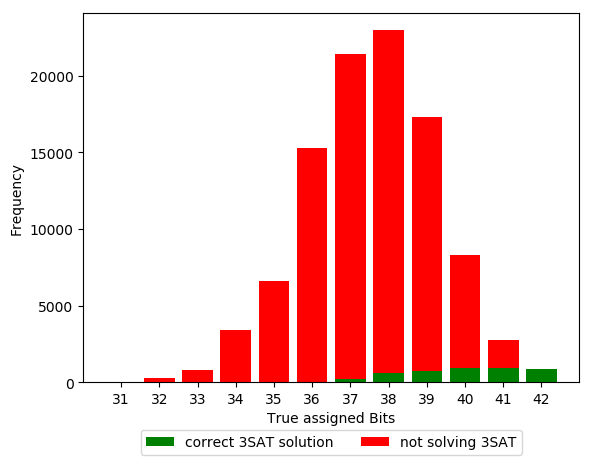
\includegraphics[width=.5\textwidth]{../material_2/Plots/42_4_2_def_engl_color_ohne_transform.png}%
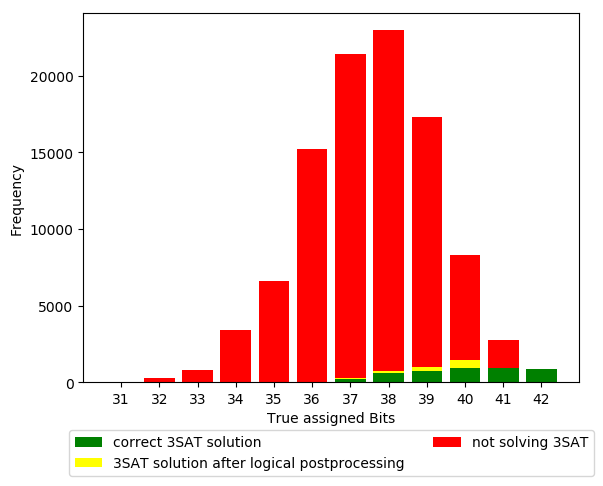
\includegraphics[width=.5\textwidth]{../material_2/Plots/42_4_2_def_engl_color_mit_transform.png}
\caption{Verteilung korrekter und nicht korrekter Antwortbitstrings ohne logisches Postprocessing (links) und mit logischem Postprocessing (rechts) für 3SAT-Instanzen bestehend aus 42 Klauseln und einem K/V- Verhältnis von 4,2.} \label{fig:distr}
\end{figure}

\begin{figure}
\centering
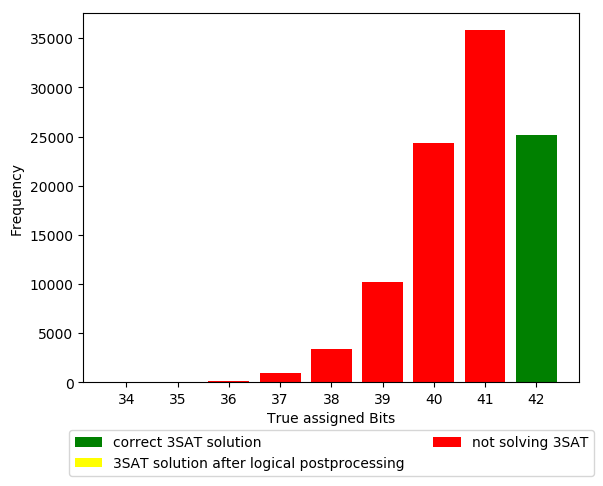
\includegraphics[width=.8\textwidth]{../material_2/Plots/42_4_2_opt_engl_color_mit_transform.png}
\caption{Verteilung korrekter und nicht korrekter Antwortbitstrings mit logischem Postprocessing für 3SAT-Instanzen bestehend aus 42 Klauseln und einem K/V- Verhältnis von 4,2.} \label{fig:distr}
\end{figure}

\begin{figure}
\centering
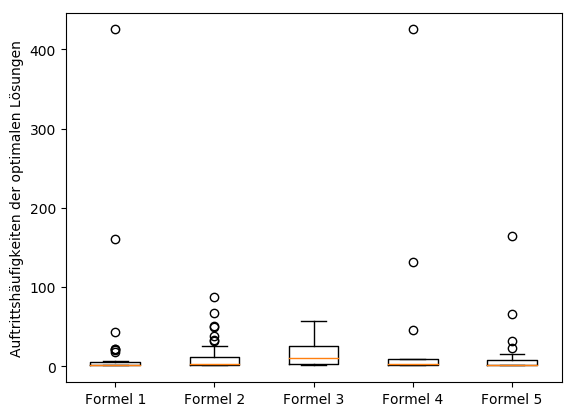
\includegraphics[width=.8\textwidth]{../material_2/25_clauses__4_2_def_MISBIAS.png}
\caption{Auftrittshäufigkeiten verschiedener optimaler Lösungen für verschiedene 3SAT-Formeln.} \label{fig:distr}
\end{figure}

\begin{figure}
\centering
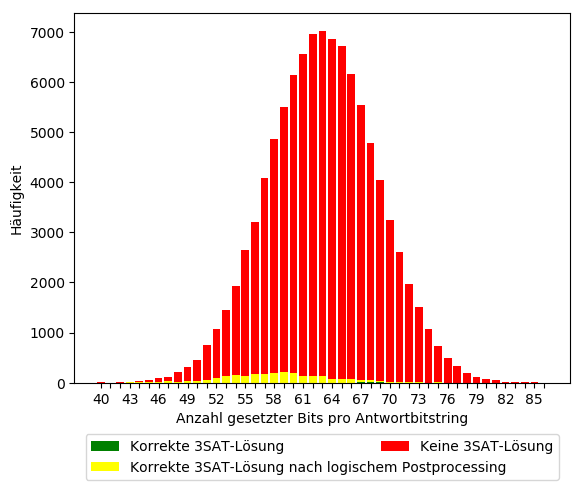
\includegraphics[width=.8\textwidth]{../material_2/42_clauses__0_2_def_RANDOM_color_transformed.png}%
%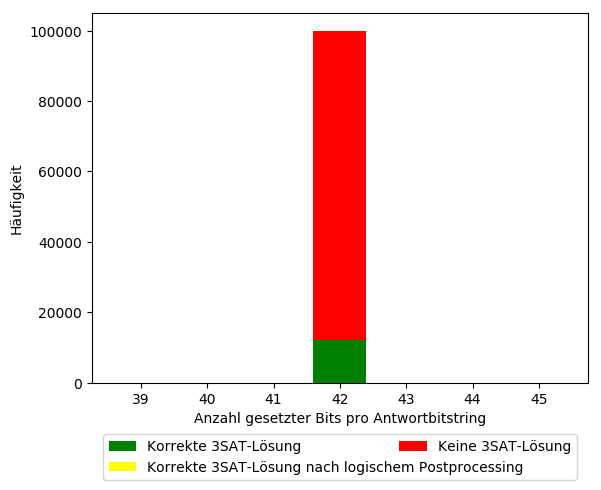
\includegraphics[width=.5\textwidth]{../material_2/42_clauses__0_2_def_RANDOM_CLEVER_color_transformed.png}
\caption{Verteilung korrekter 3SAT-Lösungen und falschen Antworten unter Ant- wortbitstrings, die durch den naiven Zufallsgenerator erzeugt wurden, mit bestimmter Anzahl gesetzter Bits für 3SAT-Formeln bestehend aus 42 Klauseln.} \label{fig:distr}
\end{figure}


\section{Conclusion}
\todo{1 Discussion \& Conclusion (7.5.3)}
%
% ---- Bibliography ----
%
% BibTeX users should specify bibliography style 'splncs04'.
% References will then be sorted and formatted in the correct style.
%
\bibliographystyle{splncs04}
\bibliography{references}
%

\end{document}
